\documentclass[letter, 10pt]{article}
\usepackage[top=2.5cm, bottom=2cm, left=2cm, right=2cm]{geometry}
\usepackage[utf8x]{inputenc}
\usepackage[spanish]{babel}
\usepackage{amsfonts}
\usepackage{amsmath}
\usepackage{graphicx}
\usepackage{color}
\usepackage{listings}

\definecolor{Code}{rgb}{0,0,0}
\definecolor{Decorators}{rgb}{0.5,0.5,0.5}
\definecolor{Numbers}{rgb}{0.5,0,0}
\definecolor{MatchingBrackets}{rgb}{0.25,0.5,0.5}
\definecolor{Keywords}{rgb}{0,0,1}
\definecolor{self}{rgb}{0,0,0}
\definecolor{Strings}{rgb}{0,0.63,0}
\definecolor{Comments}{rgb}{0.3,0.3,0.3}
\definecolor{Backquotes}{rgb}{0,0,0}
\definecolor{Classname}{rgb}{0,0,0}
\definecolor{FunctionName}{rgb}{0,0,0}
\definecolor{Operators}{rgb}{0,0,0}
\definecolor{Background}{rgb}{0.98,0.98,0.98}

\lstnewenvironment{python}[1][]{
\lstset{
numbers=left,
numberstyle=\footnotesize,
numbersep=1em,
xleftmargin=1em,
framextopmargin=2em,
framexbottommargin=2em,
showspaces=false,
showtabs=false,
showstringspaces=false,
frame=l,
tabsize=4,
% Basic
basicstyle=\ttfamily\small\setstretch{1},
backgroundcolor=\color{Background},
language=Python,
% Comments
commentstyle=\color{Comments}\slshape,
% Strings
stringstyle=\color{Strings},
morecomment=[s][\color{Strings}]{"""}{"""},
morecomment=[s][\color{Strings}]{'''}{'''},
% keywords
morekeywords={import,from,class,def,for,while,if,is,in,elif,else,not,and,or,print,break,continue,return,True,False,None,access,as,,del,except,exec,finally,global,import,lambda,pass,print,raise,try,assert},
keywordstyle={\color{Keywords}\bfseries},
% additional keywords
morekeywords={[2]@invariant},
keywordstyle={[2]\color{Decorators}\slshape},
emph={self},
emphstyle={\color{self}\slshape},
%
}}{}

\title{Laboratorio $\#$ 2\\
       Computaci\'on Cient\'ifica II\\}
\author{\bf Alumno: Diego Villouta Fredes\\
\bf Rol: 2773019-1}

\begin{document}

\begin{titlepage}
\maketitle
\thispagestyle{empty}
\end{titlepage}

\tableofcontents

\newpage

\section{ Introducci\'on }

\begin{itemize}

\item Hoy en d\'ia no es una novedad para nadie trabajar con softwares matem\'aticos potentes como Mathematica, Octave, Wolfram Alpha, entre otros y es interesante conocer como trabajan estos programas 'por debajo' por decirlo de alguna manera. Los m\'etodos de interpolaci\'on e integraci\'on num\'erica vistos en clases y en el presente laboratorio permiten entender de mejor manera como se realizan c\'alculos complejos de una manera m\'as simple para un computador en cuanto a procesamiento requerido . Para el desarrollo del laboratorio se utiliz\'o el lenguaje de programaci\'on conocido como Python y distintas librer\'ias que extienden su funcionamiento en el \'ambito matem\'atico. Las librer\'ias usadas para creaci\'on, c\'alculo y manipulaci\'on de operaciones, fueron Numpy y Scipy.

\item Cabe destacar que se opt\'o por usar la versi\'on 2.7 de Python ya que \'esta, si bien no es la \'ultima, est\'a dentro de las m\'as usadas y los complementos y librer\'ias adicionales trabajan mejor con esta versi\'on.

\end{itemize}

\section{ Objetivos }

\begin{itemize}
\item Implementar algoritmos de interpolaci\'on polinominal como son las diferencias divididas de newton y los splines c\'ubicos
\item Implementar algoritmos de integraci\'on num\'erica.
\item Desarrollar benchmarks para obtener resultados objetivos sobre las implementaciones realizadas.
\item Analizar resultados y concluir al respecto.
\end{itemize}

\newpage

\section{ Desarrollo }

\subsection{Pregunta 1}\\
\subsubsection{Funci\'on inter\_pol()} Se cre\'o la siguiente funci\'on llamada inter\_pol(x\_int, n, 'pol'), la cual retorna el valor y\_int que corresponde al valor de x\_int evaluado en el polinomio interpolador encontrado seg\'un el metodo 'pol' que se haya escogido.

\begin{itemize}
\item El c\'odigo de inter\_pol(x\_int, n, 'pol') a continuaci\'on:

\begin{python}
def inter_pol(x_int, n, pol):
#Se generan los vectores X e Y que contienen los datos para realizar la
#interpolacion.
	x,y = generate_Data(n)

#Luego se llama a las funciones interpoladores disponibles segun se haya
#escogido en un principio.
	if pol == 'diff':        
		return diff(x_int, x, y, n)
            
	if pol == 'spl':        
		return splines(x_int, x, y, n)
\end{python}

\item Se crearon 4 funciones m\'as aparte de la pedida, las cuales ser\'an detalladas a continuaci\'on. Su creaci\'on fue con la finalidad de modularizar el funcionamiento del programa y poder facilitar la programaci\'on del mismo.

\begin{enumerate}
\item \underline{generate\_Data(n):} Recibe un entero $n$ que corresponde a la cantidad de datos deseada y retorna los vectores X e Y con los datos a ser interpolados. Los valores de X est\'an en el rango [-1, 1], por condiciones del problema, y est\'an equiespaciados entre si. El c\'odigo a continuaci\'on:

\begin{python}
def generate_Data(n):
#Se crea el vector X con n datos equiespaciados entre si, que pertenecen
#al rango [-1,1].
	x = sp.linspace(-1,1,n)

#Se genera el vector Y con n datos, correspondientes a evaluar los valores
#de X en la funcion original.
	y = []    
    
	for i in range(n): 
        
		num = float(10*sp.log10(x[i]**2 + x[i] + 1))
		den = float(10*(x[i]**3) - 20*(x[i]**2) + x[i] - 2)
		y.append(float(num/den))
    
	return x, y
\end{python}

\item \underline{get\_Yreal(x):} Recibe un valor num\'erico en particular para ser evaluado en la funci\'on original y retorna su valor. El c\'odigo a continuaci\'on:

\begin{python}
def get_Yreal(x):
#Se evalua la funcion original en el valor x recibido.
	num = float(10*sp.log10(x**2 + x + 1))
	den = float(10*(x**3) - 20*(x**2) + x - 2)

	return float(num/den)
\end{python}

\newpage

\item \underline{diff(x\_int, x, y, n):} Funci\'on que aplica el m\'etodo de las diferencias divididas de Newton a un conjunto de datos X e Y de tama\~no $n$ para encontrar el polinomio interpolador, y finalmente evalua el valor x\_int en este y retorna su valor. El c\'odigo a continuaci\'on:

\begin{python}
def diff(x_int, x, y, n):
#Se crea un vector que contiene los mismos valores de Y, y se mantiene su
#primer valor ya que este corresponde al primer coeficiente del polinomio.
    coef = y
    n = n-1

#El metodo de las diferencias divididas se aplica a continuacion, donde se
#van restando y dividiendo los valores del vector 'coef' y de X hasta que
#todos los valores contenidos en 'coef' corresponden a los coeficientes
#finales del polinomio interpolador.
    for i in range(1, n+1):
        for j in range(n, i-1, -1):
            coef[j] = (coef[j] - coef[j-1])/(x[j] - x[j-i])

#Finalmente se evalua el valor de x_int en el polinomio de la forma
#coef[0] + coef[1](x_int - x[0]) + coef[2](x_int - x[0])(x_int - x[1])...
    resultado = coef[0]
    factor = 1
    
    for i in range(0, n):
            
        factor *= (x_int - x[i])
        resultado += factor*coef[i+1]
    
    return resultado
\end{python}

\item \underline{splines(x\_int, x, y, n):} Funci\'on que aplica el m\'etodo de los splines c\'ubicos a un conjunto de datos X e Y de tama\~no $n$ para encontrar los distintos polinomios interpoladores de grado 3 para cada subtramo [x[i], x[i+1]], finalmente se evalua el valor de x\_int en su spline c\'ubico correspondiente y se retorna su valor. La forma de calcular los splines fue extraida de la materia que se encuentra en la p\'agina oficial de la asignatura, consistente en como calcular los coeficientes $a_j$, $b_j$, $c_j$ y  $d_j$  de cada spline.

\begin{python}
def splines(x_int, x, y, n):
#Se crea una matriz de ceros, de dimensiones 'nxn' que contiene los
#terminos [1, 4, 1] a lo largo de su diagonal a excepcion de las
#casillas [0,0] y [n-1, n-1].

	A = sp.zeros((n,n))
    A[0,0] = 1
    A[n-1,n-1] = 1
    
    for i in range(1,n-1):
        A[i,i-1] = 1
        A[i,i] = 4
        A[i,i+1] = 1
#Se crea un vector de ceros, de la misma dimension que el vector Y, el
#cual tiene ceros en el primer y ultimo elemento, y el resto del vector
#posee elementos de la forma y[i-1] - 2*y[i] + y[i+1].

    Y = sp.zeros(n)
    
    for i in range(1,n-1):
        Y[i] = y[i-1] - 2*y[i] + y[i+1]
\end{python}

\newpage

\begin{python}
#Una vez que se tienen ambos elementos, A e Y, se procede a resolver el
#sistema de ecuaciones con la funcion linalg.solve(A,Y) de numpy, la que
#retorna finalmente un vector con todos los coeficientes C_j de los splines.

    C = np.linalg.solve(A,Y)

#Finalmente se debe evaluar el valor de x_int en el spline correspondiente,
#para encontrar el coeficiente C_j que le corresponde, se busca primero el
#indice del vector X del valor mas cercano a x_int y luego que se tiene este
#indice, se procede a encontrar los demas coeficientes A_j, B_j y D_j
#utilizando las formulas que aparecen en la pagina de la asignatura.
   
    index = min(range(n), key=lambda i: abs(x[i]-x_int))
    
    if index == (n-1):
        index = index - 1
    
    h = float((x[n-1] - x[0])/n)
    x_j = x[index]  
    a_j = y[index]
    c_j = C[index]    
    b_j = (y[index+1]-a_j)/h - (h*(C[index+1]+2*c_j))/3
    d_j = (C[index+1] - c_j)/(3*h)
    diff = x_int - x_j
    resultado = a_j + b_j*diff + c_j*(diff**2) + d_j*(diff**3)
    
    return resultado
\end{python}
\end{enumerate}
\end{itemize}

\subsubsection{Benchmark} Se pide un benchmark para los m\'etodos implementados, para lo que se creo una funci\'on cuyo c\'odigo es el siguiente:
\begin{itemize}
\begin{python}
def benchmark():
    
    X = [-0.5,-0.25,0.0,0.25,0.5]
    interp_methods = ['diff','spl']
    
    for m in range(1,6):
        for j in interp_methods:
            for i in X:
                
                n = 2**m
                y_real = get_Yreal(i)
                y_int = inter_pol(i,n,j)
                
                if y_real != 0:
                    error_rel = abs((y_real - y_int)/y_real)
                else:
                    error_rel = abs(y_real - y_int)
                
                comp_time = t.timeit("inter_pol(x_int,n,pol)",setup='x_int='+str(i)+'; 
n='+str(n)+'; pol="'+j+'"; from __main__ import inter_pol',number=10)
\end{python}

\newpage

\begin{python}
                if y_real == 0:
                    print 'N:',n,' X:',i,' Y_k:',y_real,'            Y_int:',y_int,' pol:',j
,' Error Relativo:',error_rel,' Tiempo de computo:',comp_time
                else:
                    print 'N:',n,' X:',i,' Y_k:',y_real,' Y_int:',y_int,' pol:',j
,' Error Relativo:',error_rel,' Tiempo de computo:',comp_time
                    
            print ''
\end{python}
\item La cual no necesita mayor explicaci\'on, genera los datos pedidos en el enunciado y los muestra por pantalla de una manera apropiada y los datos obtenidos son los siguientes:

\begin{center}
	\begin{tabular}{|c|c|c|c|c|c|c|}
		\hline
		$n$ & $x$ & $y_k = f(x)$ & y\_int & pol & \textbf{Error relativo} & \textbf{Tiempo de c\'omputo} \\
		\hline \hline
		
			& $ -1/2 $ & $ 0.142787127552 $ & $ -0.1084366488 $ &  diff  & $ 1.75942874304 $ & $ 0.00274220982076 $ \\ 
			& $ -1/4 $ & $ 0.246636937707 $ & $ -0.1626549732 $ &  diff  & $ 1.65949153729 $ & $ 0.0025914331928 $ \\ 
		$2$ & $ 0 $ & $ -0.0 $ & $ -0.2168732976 $ &  diff  & $ 0.2168732976 $ & $ 0.00261068127297 $ \\ 
			& $ 1/4 $ & $ -0.41529428423 $ & $ -0.271091622 $ &  diff  & $ 0.347230067223 $ & $ 0.00259207479547 $ \\ 
			& $ 1/2 $ & $ -0.462929616545 $ & $ -0.3253099464 $ &  diff  & $ 0.297279900069 $ & $ 0.00270243045508 $ \\
		\hline
		
			& $ -1/2 $ & $ 0.142787127552 $ & $ -0.2168732976 $ &  spl  & $ 2.51885748609 $ & $ 0.00428398104192 $ \\ 
			& $ -1/4 $ & $ 0.246636937707 $ & $ -0.3253099464 $ &  spl  & $ 2.31898307457 $ & $ 0.00482870171058 $ \\ 
		$2$ & $ 0 $ & $ -0.0 $ & $ -0.4337465952 $ &  spl  & $ 0.4337465952 $ & $ 0.00470230598416 $ \\ 
			& $ 1/4 $ & $ -0.41529428423 $ & $ -0.542183244 $ &  spl  & $ 0.305539865555 $ & $ 0.00493392454881 $ \\ 
			& $ 1/2 $ & $ -0.462929616545 $ & $ -0.6506198928 $ &  spl  & $ 0.405440199862 $ & $ 0.00490761883925 $ \\ 

		\hline \hline
			& $ -1/2 $ & $ 0.142787127552 $ & $ 0.312487149145 $ &  diff  & $ 1.18848263497 $ & $ 0.0076292973745 $ \\ 
			& $ -1/4 $ & $ 0.246636937707 $ & $ 0.153534213483 $ &  diff  & $ 0.377488972615 $ & $ 0.00745863106371 $ \\ 
		$4$ & $ 0 $ & $ -0.0 $ & $ -0.103568096603 $ &  diff  & $ 0.103568096603 $ & $ 0.0121031928074 $ \\ 
			& $ 1/4 $ & $ -0.41529428423 $ & $ -0.374833556813 $ &  diff  & $ 0.0974266416695 $ & $ 0.00596305523493 $ \\ 
			& $ 1/2 $ & $ -0.462929616545 $ & $ -0.576275942849 $ &  diff  & $ 0.244845700626 $ & $ 0.00502439052558 $ \\
		\hline
		
			& $ -1/2 $ & $ 0.142787127552 $ & $ 0.428100988728 $ &  spl  & $ 1.99817634871 $ & $ 0.00786091593914 $ \\ 
			& $ -1/4 $ & $ 0.246636937707 $ & $ 0.11174267883 $ &  spl  & $ 0.546934535155 $ & $ 0.00800655974572 $ \\ 
		$4$ & $ 0 $ & $ -0.0 $ & $ -0.406746663492 $ &  spl  & $ 0.406746663492 $ & $ 0.00652894879177 $ \\ 
			& $ 1/4 $ & $ -0.41529428423 $ & $ -0.448631458742 $ &  spl  & $ 0.0802736174752 $ & $ 0.00627551573627 $ \\ 
			& $ 1/2 $ & $ -0.462929616545 $ & $ -0.454744096152 $ &  spl  & $ 0.0176819976522 $ & $ 0.00708072708981 $ \\ 

		\hline \hline
			& $ -1/2 $ & $ 0.142787127552 $ & $ 0.0938597561839 $ &  diff  & $ 0.342659539464 $ & $ 0.00942899286987 $ \\ 
			& $ -1/4 $ & $ 0.246636937707 $ & $ 0.290706461664 $ &  diff  & $ 0.178681767489 $ & $ 0.0097921399823 $ \\ 
		$8$ & $ 0 $ & $ -0.0 $ & $ -0.0177906159806 $ &  diff  & $ 0.0177906159806 $ & $ 0.0121025512047 $ \\ 
			& $ 1/4 $ & $ -0.41529428423 $ & $ -0.434838969532 $ &  diff  & $ 0.0470622545109 $ & $ 0.00944374973133 $ \\ 
			& $ 1/2 $ & $ -0.462929616545 $ & $ -0.429838614744 $ &  diff  & $ 0.0714817125939 $ & $ 0.0104837876629 $ \\
		\hline
		
			& $ -1/2 $ & $ 0.142787127552 $ & $ 0.164302232108 $ &  spl  & $ 0.150679581027 $ & $ 0.0117625017885 $ \\ 
			& $ -1/4 $ & $ 0.246636937707 $ & $ 0.43541685672 $ &  spl  & $ 0.765416246115 $ & $ 0.0118600253946 $ \\ 
		$8$ & $ 0 $ & $ -0.0 $ & $ -0.189495703506 $ &  spl  & $ 0.189495703506 $ & $ 0.011630331638 $ \\ 
			& $ 1/4 $ & $ -0.41529428423 $ & $ -0.368404518462 $ &  spl  & $ 0.112907322708 $ & $ 0.0112909238244 $ \\ 
			& $ 1/2 $ & $ -0.462929616545 $ & $ -0.458927916166 $ &  spl  & $ 0.00864429545274 $ & $ 0.0193199396637 $ \\ 

		\hline
	\end{tabular}
\end{center}

\begin{center}
	\begin{tabular}{|c|c|c|c|c|c|c|}
		\hline
		$n$ & $x$ & $y_k = f(x)$ & y\_int & pol & \textbf{Error relativo} & \textbf{Tiempo de c\'omputo} \\
		\hline \hline
			& $ -1/2 $ & $ 0.142787127552 $ & $ 0.138944204909 $ &  diff  & $ 0.0269136490756 $ & $ 0.023808591958 $ \\ 
			& $ -1/4 $ & $ 0.246636937707 $ & $ 0.245061304459 $ &  diff  & $ 0.00638847231247 $ & $ 0.0311543009514 $ \\ 
		$16$& $ 0 $ & $ -0.0 $ & $ -0.000494705457066 $ &  diff  & $ 0.000494705457066 $ & $ 0.0216220100513 $ \\ 
			& $ 1/4 $ & $ -0.41529428423 $ & $ -0.414594674005 $ &  diff  & $ 0.00168461318058 $ & $ 0.0319453970462 $ \\ 
			& $ 1/2 $ & $ -0.462929616545 $ & $ -0.460327445613 $ &  diff  & $ 0.00562109409103 $ & $ 0.0226537071482 $ \\
		\hline
		
			& $ -1/2 $ & $ 0.142787127552 $ & $ 0.141770752843 $ &  spl  & $ 0.00711811160101 $ & $ 0.0198184649399 $ \\ 
			& $ -1/4 $ & $ 0.246636937707 $ & $ 0.292242991092 $ &  spl  & $ 0.184911691691 $ & $ 0.0192981251728 $ \\ 
		$16$& $ 0 $ & $ -0.0 $ & $ -0.0184401735992 $ &  spl  & $ 0.0184401735992 $ & $ 0.0256718061179 $ \\ 
			& $ 1/4 $ & $ -0.41529428423 $ & $ -0.404061996171 $ &  spl  & $ 0.0270465751299 $ & $ 0.0206685884805 $ \\ 
			& $ 1/2 $ & $ -0.462929616545 $ & $ -0.461843181556 $ &  spl  & $ 0.00234686861852 $ & $ 0.0190896043044 $ \\

		\hline \hline
			& $ -1/2 $ & $ 0.142787127552 $ & $ 0.1427630408 $ &  diff  & $ 0.000168689941292 $ & $ 0.0533030667966 $ \\ 
			& $ -1/4 $ & $ 0.246636937707 $ & $ 0.246634912923 $ &  diff  & $ 8.20957485681e-06 $ & $ 0.0533332221222 $ \\ 
		$32$& $ 0 $ & $ -0.0 $ & $ -3.83824555686e-07 $ &  diff  & $ 3.83824555686e-07 $ & $ 0.0542398066979 $ \\ 
			& $ 1/4 $ & $ -0.41529428423 $ & $ -0.415293385191 $ &  diff  & $ 2.16482445618e-06 $ & $ 0.0524336951759 $ \\ 
			& $ 1/2 $ & $ -0.462929616545 $ & $ -0.462913306652 $ &  diff  & $ 3.52319070007e-05 $ & $ 0.0734756964116 $ \\
		\hline
		
			& $ -1/2 $ & $ 0.142787127552 $ & $ 0.142300374891 $ &  spl  & $ 0.00340893937324 $ & $ 0.0370531959192 $ \\ 
			& $ -1/4 $ & $ 0.246636937707 $ & $ 0.254704980693 $ &  spl  & $ 0.032712224944 $ & $ 0.0448563676178 $ \\ 
		$32$& $ 0 $ & $ -0.0 $ & $ -0.00446981582699 $ &  spl  & $ 0.00446981582699 $ & $ 0.0359053687387 $ \\ 
			& $ 1/4 $ & $ -0.41529428423 $ & $ -0.412571540349 $ &  spl  & $ 0.00655617951974 $ & $ 0.0470756712608 $ \\ 
			& $ 1/2 $ & $ -0.462929616545 $ & $ -0.462646295074 $ &  spl  & $ 0.000612018460719 $ & $ 0.0390158584932 $ \\

		\hline
	\end{tabular}
\end{center}

\end{itemize}

\subsection{Pregunta 2}\\
\subsubsection{Funci\'on erf\_teo(y, n)} Antes de explicar la funci\'on erf\_teo(y, n), se explicar\'an dos simples funciones m\'as:

\begin{itemize}
\item \underline{get\_roots(n)}: Recibe un n\'umero entero $n$ que corresponde al grado del Polinomio de Legendre a utilizar, el cual por condici\'on del laboratorio debe estar en $4 \leq n \leq 7$, y usando la funci\'on 'scipy.special.orthogonal.p\_roots(n)[0]', se obtiene un arreglo con las raices del Polinomio de Legendre de grado $n$. El c\'odigo a continuaci\'on:

\begin{python}
import scipy.special as sps

def get_roots(n):
    
    return sps.orthogonal.p_roots(n)[0]
\end{python}

\item \underline{get\_coefs(n)}: Recibe un n\'umero entero $n$ que corresponde al grado del Polinomio de Legendre a utilizar, el cual por condici\'on del laboratorio debe estar en $4 \leq n \leq 7$, y usando la funci\'on 'scipy.special.orthogonal.p\_roots(n)[1]', se obtiene un arreglo con los coeficientes $C_i$ asociados a las raices del Polinomio de Legendre de grado $n$. El c\'odigo a continuaci\'on:

\begin{python}
import scipy.special as sps

def get_coefs(n):        
    
    return sps.orthogonal.p_roots(n)[1]
\end{python}

\newpage

\item Luego de explicar las dos funciones anteriores, es posible explicar la funci\'on pedida en un comienzo, $erf\_teo(y, n)$, la cual recibe como par\'ametros $y$, que corresponde al l\'imite superior de la integral $erf(y)$, y $n$ que corresponde al grado del Polinomio de Legendre, cuyas raices ser\'an utilizadas para el m\'etodo de la cuadratura de Gauss. El c\'odigo a continuaci\'on:

\begin{python}
import math as m

def erf_teo(y, n):

#Se comprueba que 'n' este dentro del rango pedido.
    if 4 <= n <= 7:
    
#Se obtienen las raices y los coeficientes necesarios para la cuadratura.
        x_i = get_roots(n)
        c_i = get_coefs(n)    

#La cuadratura de Gauss solo es valida en los limites de integracion [-1, 1], por
#lo que se deben cambiar los limites de la integral erf(y) a estos. Luego de
#realizar el cambio se obtiene un factor constante denominado 'factor_1'.
        factor_1 = y/m.sqrt(m.pi)
        
        res = 0
#Es en este ciclo donde se realiza la cuadratura como tal, se hace una sumatoria de
#la multiplicacion de cada coeficiente Ci por la funcion evaluada en la raiz del
#Polinomio de Legendre correspondiente. En este caso, como se debieron mover los
#limites de integracion, la funcion no se evalua directamente en las raices y ahora
#se evalua en el valor contenido por la variable 'x'.
        for i in range(n):        
            x = (y*x_i[i] + y)/2        
            res += c_i[i]*m.exp(-x**2)

#Finalmente se multiplica el resultado obtenido de la sumatoria por el factor
#constante explicado anteriormente.
        return res*factor_1
    else: 
        print 'n value out of range'
\end{python}

\end{itemize}

\subsubsection{Tabla de raices del Polinomio de Legendre} 


\begin{tabular}{|c|c|c|c|c|c|}
		\hline
		$n$ & $x_1$ & $x_2$ & $x_3$ & $x_4$ & $x_5$ \\
		\hline \hline
		$ 4 $ & $ -0.861136311594 $ & $ -0.339981043585 $ & $ 0.339981043585 $ & $ 0.861136311594 $ & $ $ \\ 
		$ 5 $ & $ -0.906179845939 $ & $ -0.538469310106 $ & $ -1.25197490269e-16 $ & $ 0.538469310106 $ & $ 0.906179845939 $ \\ 
		$ 6 $ & $ -0.932469514203 $ & $ -0.661209386466 $ & $ -0.238619186083 $ & $ 0.238619186083 $ & $ 0.661209386466 $ \\ 
		$ 7 $ & $ -0.949107912343 $ & $ -0.741531185599 $ & $ -0.405845151377 $ & $ 6.97980421714e-18 $ & $ 0.405845151377 $ \\
		\hline
\end{tabular}
	
\begin{tabular}{|c|c|c|}
		\hline
		$n$ & $x_6$ & $x_7$ \\
		\hline \hline
		$ 4 $ & $ $ & $ $ \\ 
		$ 5 $ & $ $ & $ $ \\ 
		$ 6 $ & $ 0.932469514203 $ & $ $ \\ 
		$ 7 $ & $ 0.741531185599 $ & $ 0.949107912343 $ \\
		\hline
\end{tabular}

\newpage

\subsubsection{Tabla de $c_i$ y valores de erf() obtenidos}

\begin{tabular}{|c|c|c|c|c|c|c|}
		\hline
		$n$ & $c_1$ & $c_2$ & $c_3$ & $c_4$ & $c_5$ & $c_6$ \\
		\hline \hline
		$ 4 $ & $ 0.347854845137 $ & $ 0.652145154863 $ & $ 0.652145154863 $ & $ 0.347854845137 $ & $ $ & $ $ \\ 
		$ 5 $ & $ 0.236926885056 $ & $ 0.478628670499 $ & $ 0.568888888889 $ & $ 0.478628670499 $ & $ 0.236926885056 $ & $ $ \\ 
		$ 6 $ & $ 0.171324492379 $ & $ 0.360761573048 $ & $ 0.467913934573 $ & $ 0.467913934573 $ & $ 0.360761573048 $ & $ 0.171324492379 $ \\ 
		$ 7 $ & $ 0.129484966169 $ & $ 0.279705391489 $ & $ 0.381830050505 $ & $ 0.417959183673 $ & $ 0.381830050505 $ & $ 0.279705391489 $ \\
		\hline
\end{tabular}

\begin{tabular}{|c|c|c|}
		\hline
		$n$ & $c_7$ & $erf\_teo(10, n)$ \\
		\hline \hline
		$ 4 $ & $ $ & $ 1.2119475604 $ \\ 
		$ 5 $ & $ $ & $ 1.08582368212 $ \\  
		$ 6 $ & $ $ & $ 0.97790965366 $ \\
		$ 7 $ & $ 0.129484966169 $ & $ 0.982074829295 $ \\
		\hline
\end{tabular}

\subsubsection{Gr\'afico} El siguiente gr\'afico muestra como var\'ia el valor de $erf\_teo(10, n)$ a medida que el valor de n aumenta desde 4 hasta 7. Se puede apreciar que para $n = 7$, el valor se acerca m\'as a 1, que es el valor real de la funci\'on.

\begin{center}
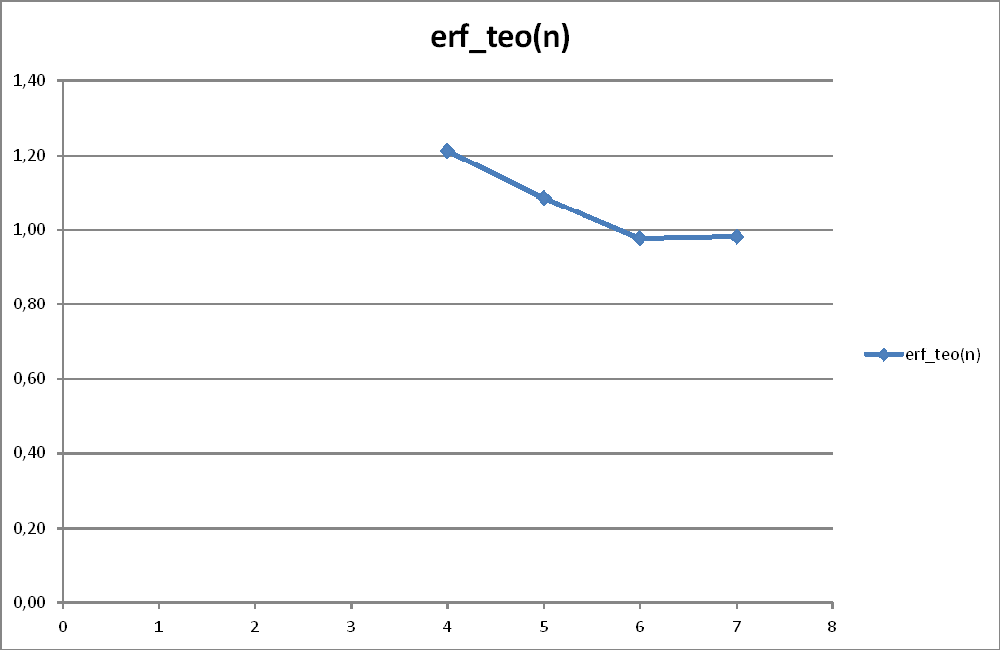
\includegraphics[width=15cm]{grafico.png}
\end{center}

\newpage

\subsubsection{Funci\'on erf\_real()} Para obtener el valor 'real' de la integral se utiliz\'o la funci\'on 'scipy.integrate.quad(func,a,b)', la cual recibe la funci\'on a integrar y los l\'imites de la integral $a$ y $b$. El c\'odigo a continuaci\'on:

\begin{python}
import scipy.integrate as spi

#Recibe como parametro el limite superior de la integral
def erf_real(y):

#factor representa la parte constante de la integral, y func es la funcion a integrar
    factor = 2/m.sqrt(m.pi)
    func = lambda x: m.exp(-x**2)

#Se utiliza scipy.integrate.quad() para obtener el valor de la integral definida entre
#[0, y].
    return factor*spi.quad(func,0,y)[0]
\end{python}

\subsubsection{Error relativo} A continuaci\'on una tabla con los valores de erf\_teo(y, n), erf\_real(y), y el error relativo entre estos. Para ambos $y = 10$.\\

\begin{tabular}{|c|c|c|c|}
		\hline
		$n$ & $erf\_teo(10, n)$ & $erf\_real(10)$ & $err\_teo\_real(10, n)$ \\
		\hline \hline
		$ 4 $ & $ 1.2119475604 $ & $ 1.0 $ & $ 0.211947560402 $ \\ 
		$ 5 $ & $ 1.08582368212 $ & $ 1.0 $ & $ 0.0858236821154 $ \\ 
		$ 6 $ & $ 0.97790965366 $ & $ 1.0 $ & $ 0.0220903463402 $ \\ 
		$ 7 $ & $ 0.982074829295 $ & $ 1.0 $ & $ 0.0179251707053 $ \\
		\hline
\end{tabular}

\newpage

\section{Conclusiones}
\begin{enumerate}
\item Sobre la primera pregunta, mirando y revisando los resultados de la tabla, se puede apreciar que el metodo de los Splines ser\'ia extra\~namente menos preciso para interpolar el polinomio que el metodo de las diferencias divididas. Digo extra\~no porque al interpolar entre tramos m\'as peque\~nos y con polinomios de solo grado 3, se debiesen obtener menos oscilaciones entre puntos, siendo as\'i un problema mejor condicionado. Tambi\'en se puede notar que para 'n'es m\'as peque\~nos, el m\'etodo de las diferencias divididas se calcula m\'as rapido y para 'n'es m\'as grandes, se calcula m\'as rapido el metodo de los Splines. Se podr\'ia concluir entonces que dejando un poco de lado la precisi\'on, la cual tampoco es mala, para grandes cantidades de datos conviene optar por la opci\'on de los Splines c\'ubicos para interpolar datos, pensando que el tiempo es un par\'ametro m\'as cr\'itico que la precisi\'on.\\

\item Sobre la segunda pregunta, la tabla m\'as importante es donde se compara el valor teorico con el valor real de la integral, donde se aprecia que incluso con 4 raices del polinomio, ya se obtiene una aproximaci\'on decente con un $21\%$ de error relativo, y que al aumentar a 7 raices, el error ya disminuye bastante llegando a tan solo un $1,79\%$. Se puede concluir que el m\'etodo es bastante exacto y que como el grado con mayor exactitud es de 7, la funci\'on integrada podr\'ia considerarse como un polinomio de grado hasta $2n-1$, es decir, $2*7-1$ $=$ 13.\\
\end{enumerate}

\section{Anexos}
\begin{enumerate}
\item No es necesario poner anexos ya que cada input de prueba y su respectivo output ya est\'an presentes en el informe a modo de tablas respondiendo a las preguntas del mismo.
\end{enumerate}
\end{document}